\documentclass{beamer}

% Packages
\usepackage{graphicx}   % For including images
\usepackage{amsmath}    % For math formatting
\usepackage{hyperref}   % For clickable links
\usepackage{multicol}   % For multiple columns on slides
\usepackage{xcolor}

\newcommand{\highlightred}[1]{\textcolor{red}{\textbf{#1}}}

% Title, Author, Date
\title{TA Review 5}
\author{Portfolio and Risk Management}
\date{\today}

% Begin Document
\begin{document}

% Title Slide
\begin{frame}
    \titlepage
\end{frame}

% Table of Contents Slide
\begin{frame}{Tentative Schedule}
    \tableofcontents
\end{frame}

% Section 1
\section{Pricing Factors}
\begin{frame}{Pricing Factors}
    \begin{itemize}
        \item Pricing Models are models about expected returns.
        \item Pricing Models claim that they can estimate the expected return of any asset with a set of factors.
        \item In the CAPM:
        $$
        \mathbb{E}[\tilde{r}^i] = \beta_{i, m} \mathbb{E}[\tilde{r}^m] 
        $$
        \item $\beta_{i, m}$ shows the relation between the factor and the expected return of asset $i$.
    \end{itemize}
\end{frame}

\begin{frame}{Pricing Factors}
    \begin{itemize}
        \item If we our model is about expected returns, why are we using historical returns?
        \begin{itemize}
            \item Because we need to estimate $\hat{\beta}_{i, m}$
            \item Because it gives us the possibility to test the assumption.
        \end{itemize}
    \end{itemize}
\end{frame}

\begin{frame}{Pricing Factors}
    \begin{itemize}
        \item If we our model is about expected returns, why are we using historical returns?
        \begin{itemize}
            \item Because we need to estimate $\hat{\beta}_{i, m}$
            \item Because it gives us the possibility to test the assumption of the pricing model.
        \end{itemize}
    \end{itemize}
\end{frame}

\begin{frame}{Pricing Factors}
    \begin{itemize}
        \item In the CAPM,
        $$
        \mathbb{E}[\tilde{r}^i] = \beta_{i, m} \mathbb{E}[\tilde{r}^m] 
        $$
        becomes:
        $$
        \tilde{r}^i_t = \beta_{i, m} \tilde{r}^m_t + \varepsilon_t, \quad \text{where} \quad \mathbb{E}[\varepsilon_t] = 0
        $$
        Which finally allows us to estimate $\hat{\beta}_{i, m}$
        \item But... should I care about the $\hat{\beta}_{i, m}$ of the model?
    \end{itemize}
\end{frame}

\begin{frame}{Factor Model User}
    \begin{itemize}
        \item But... should I care about the $\hat{\beta}_{i, m}$ of the model?
        \item Model User
        \begin{itemize}
            \item If I am an user of the model (if I believe the model is well specified) I mainly care about the $\hat{\beta}_{i, m}$. The $\hat{\beta}_{i, m}$ 
            \item The $\hat{\beta}_{i, m}$ gives the expected return for ANY asset.
        \end{itemize}
    \end{itemize}
\end{frame}

\begin{frame}{Factor Model Tester}
    \begin{itemize}
        \item But... should I care about the $\hat{\beta}_{i, m}$ of the model?
        \item Testing the Model
        \begin{itemize}
            \item If I am testing the model, I mainly care about knowing if it is well specified.
            \item Our specification for the CAPM:
            $$
            \tilde{r}^i_t = \beta_{i, m} \tilde{r}^m_t + \varepsilon_t, \quad \text{where} \quad \mathbb{E}[\varepsilon_t] = 0
            $$
            Meaning, that any other parameter added should not be significant (for a large enough unbiased sample) to explain returns for asset $i$. Specially an intercept...
        \end{itemize}
    \end{itemize}
\end{frame}

\begin{frame}{Factor Model Tester}
    \begin{itemize}
    \item We can test if the data generating process assumed by the CAPM holds in the data by running the regression with an intercept:
    $$
    \tilde{r}^i_t = \alpha_{i} + \beta_{i, m} \tilde{r}^m_t + \varepsilon_t
    $$
    \item If the CAPM holds, what should $\alpha_{i}$ be?
    \end{itemize}
\end{frame}

\begin{frame}{Factor Model Tester}
    \begin{itemize}
    \item $\alpha_{i}$ should be zero in population (or statistically non-significant in the sample).
    \item If $\alpha_{i}$ is not zero, it means that there is excess return not explained by the model.
    \item \highlightred{Show linear regression animation.}
    \end{itemize}
\end{frame}

\begin{frame}{Factor Model Tester}
    \begin{itemize}
        \item Recap: as a tester of the factor model, I worry about assuring that the suggested model holds.
        \item Adding an $\alpha_{i}$ allows us to check if there is, on average, excess return not related to the factor(s).
    \end{itemize}
\end{frame}

\begin{frame}{Factor Model Tester}
    \begin{itemize}
        \item Factor Pricing Models claim to price every single asset (bold claim, right?).
        \item Therefore, we should test them broadly (not for a single asset).
    \end{itemize}
\end{frame}

\section{Pricing Models vs LFD}
\begin{frame}{Pricing Models vs LFD in the Time-Series}
    \begin{itemize}
        \item We use regression for Pricing Models and LFD.
        \item LFD is about historical returns.
        \item Pricing Models are about expected returns.
    \end{itemize}
\end{frame}

\begin{frame}{Pricing Models vs LFD in the Time-Series}
What should we care about $R^2$ in LFD and Pricing?
    \begin{itemize}
        \item In the time-series analysis of a factor model, is it a problem to have $R^2 = 0$ when we are testing it?
        \item What about when we are using it?
        \item In the LFD, is it a problem to have $R^2 = 0$? 
    \end{itemize}
\end{frame}

\begin{frame}{Pricing Models vs LFD in the Time-Series}
    \begin{itemize}
        \item In the time-series analysis of a factor model, is it a problem to have $R^2 = 0$ when we are testing it? \textbf{No. It means that your $\beta_{i, m} = 0$. As long as the asset expected return is the risk-free rate (there is no excess return for the asset, $\alpha_i = 0$), the model does not present issues.}
        \item What about when we are using it? \textbf{No. It means that your $\beta_{i, m} = 0$. It means that the expected return of the asset is the risk-free rate, meaning that you do not have a very attractive asset at hand.}
    \end{itemize}
\end{frame}

\begin{frame}{Pricing Models vs LFD in the Time-Series}
    \begin{itemize}
        \item In the LFD, is it a problem to have $R^2 = 0$? \textbf{Yes. It means that your regressors are not able to capture variability of the target asset. If you are hedging, you are not able to hedge any risk. If you are tracking, your tracking instrument is expected to have a very poor performance}
    \end{itemize}
\end{frame}

\begin{frame}{Pricing Models vs LFD in the Time-Series}
        Should we care about $\alpha_i$ in LFD and Pricing?
        \begin{itemize}
            \item In the time-series analysis of a factor model, is it a problem to have $\alpha_i \neq 0$ when we are testing it?
            \item What about when we are using it?
            \item In the LFD, is it a problem to have $\alpha_i \neq 0$? 
        \end{itemize}
\end{frame}

\begin{frame}{Pricing Models vs LFD in the Time-Series}
    \begin{itemize}
        \item In the time-series analysis of a factor model, is it a problem to have $\alpha_i \neq 0$ when we are testing it? \textbf{Yes. it means that the asset is, on average, getting compensated more/less than the risk-free due to risk non-associated with the factor(s).}
        \item What about when we are using it? \textbf{You should not use an alpha in your regressor.}
        \item In the LFD, is it a problem to have $\alpha_i \neq 0$? \textbf{No. But the meaning you give to this $\alpha_i$ will help you decide how to use it in the regression.}
    \end{itemize}
\end{frame}

\begin{frame}{Pricing Models vs LFD in the Time-Series}
    Should we care about $\beta_{m, i}$ in LFD and Pricing?
    \begin{itemize}
        \item In the time-series analysis of a factor model, should I care about $\beta_{m, i}$ when we are testing it?
        \item What about when we are using it?
        \item In the LFD, should I care about $\beta_{m, i}$?
    \end{itemize}
\end{frame}

\begin{frame}{Pricing Models vs LFD in the Time-Series}
    \begin{itemize}
        \item In the time-series analysis of a factor model, should I care about $\beta_{m, i}$ when we are testing it? \textbf{No, only $\alpha_i$}
        \item What about when we are using it? \textbf{Yes. It will give you the expected return of the asset.}
        \item In the LFD, should I care about $\beta_{m, i}$? \textbf{Yes. It will give you exposure when assessing performance and positions when tracking and hedge}
    \end{itemize}
\end{frame}

\section{Testing a Pricing Model}
\begin{frame}{Testing a Pricing Model}
    \begin{itemize}
        \item All that was mentioned before holds for multifactor models.
        \item ...Now, how to properly to test a factor model?
        \begin{enumerate}
            \item Select $n$ test assets.
            \item Run $n$ time-series regressions.
            \item From here, you can either:
            \begin{itemize}
                \item Check the $\alpha_i$ values.
                \item Run 1 cross-sectional regression.
            \end{itemize}
        \end{enumerate}
        \highlightred{To the board...}
    \end{itemize}
\end{frame}

\begin{frame}{Testing a Pricing Model}
    Consider a factor model with $p$ factors

    \textcolor{red}{Estimated by the regression in red}
    \begin{itemize}
        \item Time-Series: \[
            \tilde{r}^i_t=\textcolor{red}{\alpha}+\textcolor{red}{\beta^{i, 1}} \tilde{r}^1_t+\textcolor{red}{\beta^{i, 2}} \tilde{r}^2_t+\ldots+\textcolor{red}{\beta^{i, p}} \tilde{r}^n_t+\varepsilon_i
            \]
        \item Cross-Section: \[
            \mathbb{E}[\tilde{r}^i]=\textcolor{red}{\eta}+\beta^{i, 1}\textcolor{red}{\lambda_{1}}+\beta^{i, 2}\textcolor{red}{\lambda_{2}}+...+\beta^{i, p}\textcolor{red}{\lambda_{n}}+\nu_i
            \]
    \end{itemize}
    \begin{table}[h]
        \centering
        \begin{tabular}{|l|c|c|}
            \hline
            \textbf{Metric} & \textbf{Time-Series} & \textbf{Cross Sectional} \\ \hline
            $R^2$ & not important & important \\ \hline
            Intercept & ($\alpha_i$) important & ($\eta$) important \\ \hline
            MAE & $\frac{1}{n} \sum_{i=1}^{n} | \alpha_i |$ & $\frac{1}{n}  \sum_{i=1}^{n} | \nu_i |$ \\ \hline
            Estimated & $\beta_{i, m}$ & $\lambda_m$ \\ \hline
            Risk-Premia of Factor & $\overline{\tilde{r}}_m$ (avg) & $\lambda_m$ \\ \hline
        \end{tabular}
        \caption{Importance of Metrics for Pricing Model Tests}
        \label{tab:importance_of_metrics}
    \end{table}
\end{frame}

\section{Other Important Points}
\begin{frame}{Other Important Points}
    \begin{itemize}
        \item \highlightred{Go to report}
    \end{itemize}
\end{frame}

\section{AQR Value Spread}
\begin{frame}{AQR Value Spread}
    \begin{figure}[h]
    \centering
        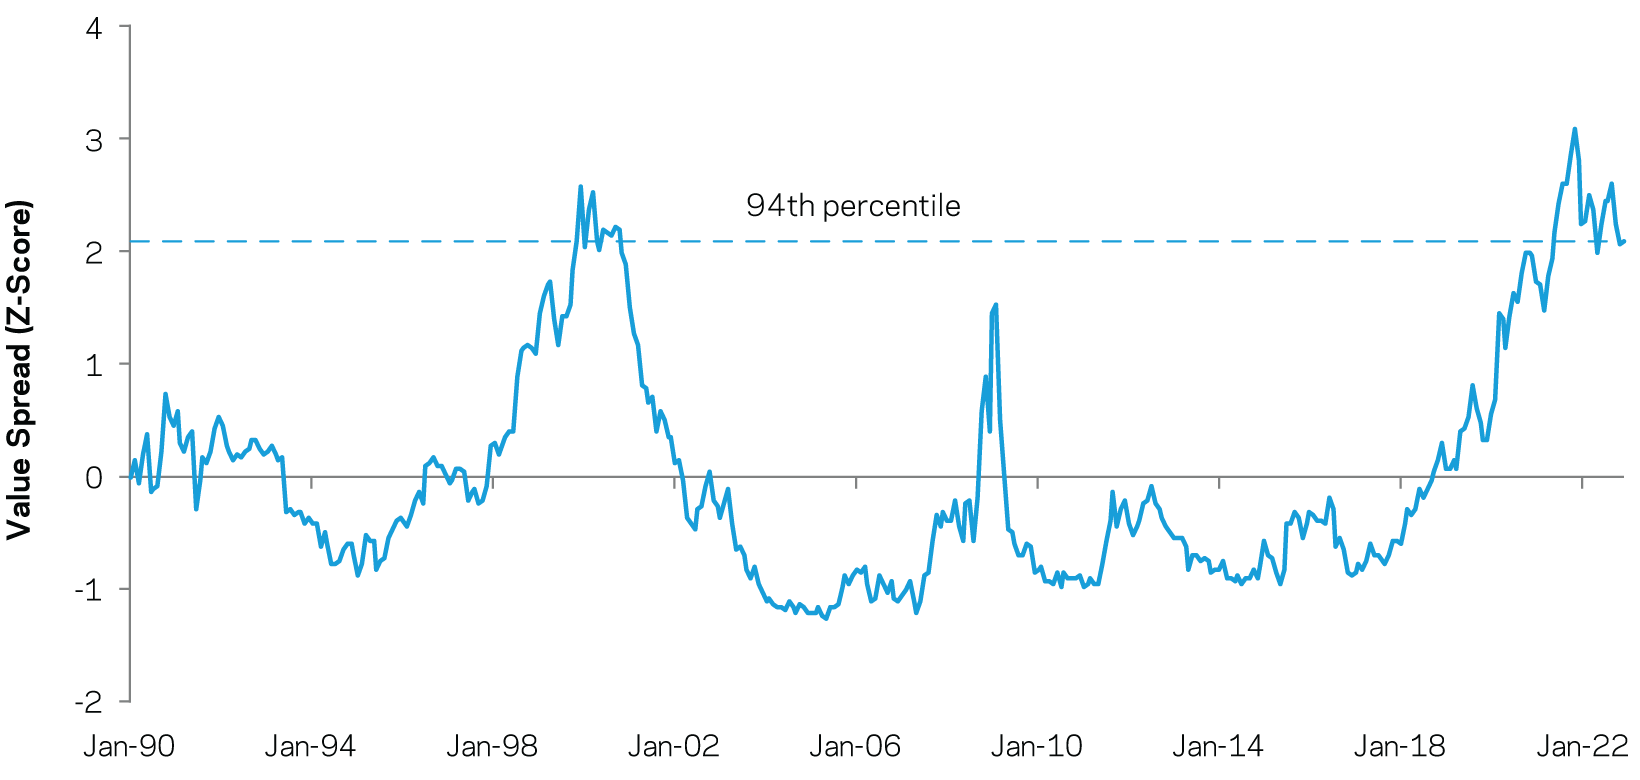
\includegraphics[width=1\textwidth]{value_spread.png}
        \caption{Value Spread: Avg Valuation of "Growth" Stock - Avg Valuation of "Value" Stock}
        \label{fig:sample_image}
    \end{figure}
    \begin{itemize}
        \item Unconditional vs Conditional Expected Return of a Factor?
    \end{itemize}
\end{frame}

\begin{frame}{AQR Timing?}
    \begin{itemize}
        \item Market Timing: Sin a Little
        
        \url{https://www.aqr.com/Insights/Research/Journal-Article/Market-Timing-Sin-a-Little}
    \end{itemize}
\end{frame}

\section{Midterm 1 Review}
\begin{frame}{Midterm 1 Solutions Review}
    \begin{itemize}
        \item \highlightred{Go to midterm solutions}
    \end{itemize}
\end{frame}

\section{Unconditional vs Conditional Sorting}
\begin{frame}{Unconditional vs Conditional Test Assets}
    \begin{itemize}
        \item Forest Through the Trees: Building Cross-Sections of Stock Returns
        
        \url{https://papers.ssrn.com/sol3/papers.cfm?abstract_id=3493458}
        
        \item Replication
        
        \url{https://github.com/Fernando-Urbano/forest-through-the-trees/blob/main/README.md}
    \end{itemize}
\end{frame}

\section{Homework 5}
\begin{frame}{Homework 5}
    \begin{itemize}
        \item \highlightred{Go to homework 5}
    \end{itemize}
\end{frame}

\end{document}